\section{Definitions and Problem Statement}
\seclabel{problem}

Given a previously unknown object, we consider the problem of finding the parallel-jaw grasp with the maximum expected grasp quality according to a binary grasp quality metric such as force closure under uncertainty in object pose, gripper pose, and friction coefficient.

\subsection{Grasp and Object Model}
Our grasping model is illustrated in~\figref{grasp-model}.
Let $\bg = [\bx, \bw]^T$ be a parallel-jaw grasp parameterized by the centroid of the jaws in 3D space $\bx \in \mathbb{R}^3$ and an approach direction, or axis, $\bv \in \bS^2$.
We assume that the jaws are opened to their maximal width $w \in\bR$ before closing on the object.
Let $f: \mathbb{R}^3 \rightarrow \mathbb{R}$ be a signed distance function (SDF) representing an object's geometry~\cite{mahler2015gp, newcombe2011kinectfusion}, which is zero on the object surface, positive outside the object, and zero inside the object. 
We assume that the object is specified in units of meters and the object center of mass $\bz \in \mathbb{R}^3$ is known.
Let $\mG = \{ [\bx, \bw]^T \big| \bx \in \mathbb{R}^3, \bv \in \bS^2\}$ denote the space of all grasps and $\mH = \{ \mO = \{\bz, f(\cdot)\} \big|  \bz \in \mathbb{R}^3, f \in \mF\}$ denote the space of all objects, where $\mF$ is the space of all SDFs.
Our joint space of grasps and objects, or Grasp Moduli Space~\cite{pokorny2013grasp}, is $\mM = \mG \times \mH$.

\begin{figure}[t!]
\centering
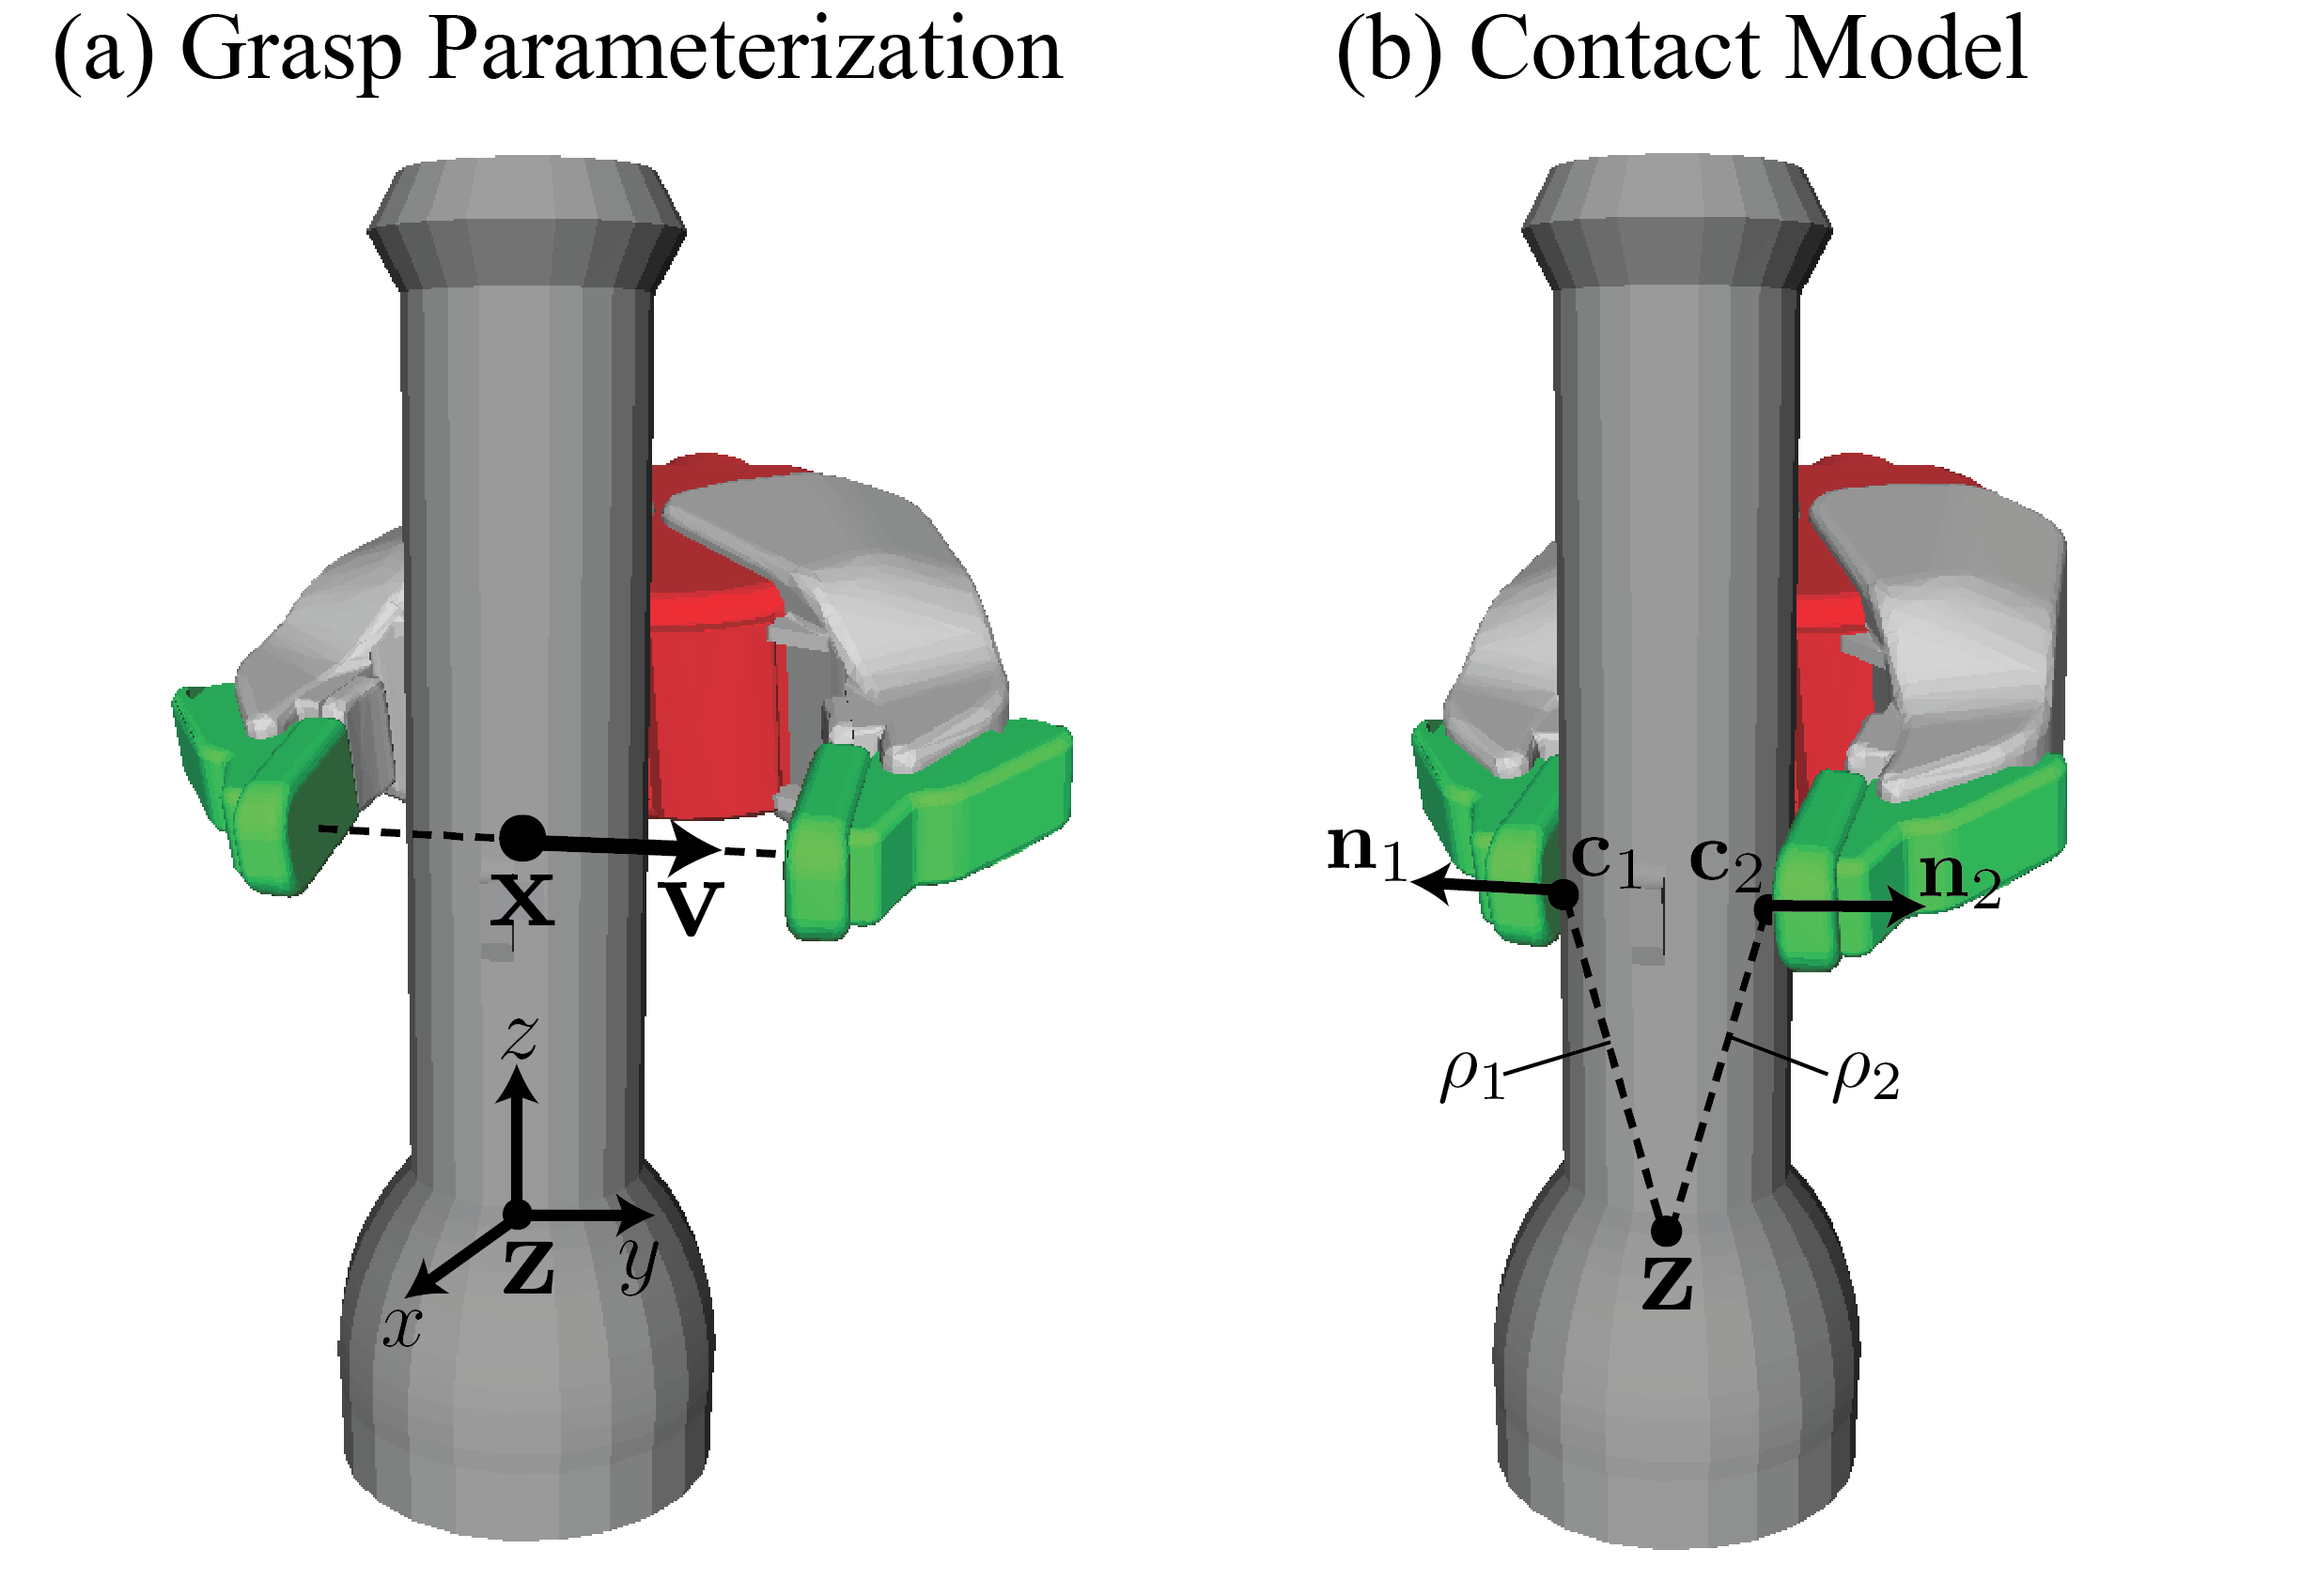
\includegraphics[scale=0.4]{figures/illustrations/dexnet_grasping_model.png}
\caption{(Left) We parameterize parallel-jaw grasps by the centroid of the jaws $\bx \in \mathbb{R}^3$ and approach direction, or direction along which the jaws close, $\bv \in \mS^2$. The grasp parameters $\bx$ and $\bv$ are specified with respect to a coordinate frame located at the object center of mass $\bz$ and oriented along the principal directions of the object. (Right) The jaws are closed until contacting the object surface at locations $\bc_1, \bc_2 \in \mathbb{R}^3$, at which the surface has normals $\bn_1, \bn_2 \in \mathbb{S}^2$. The contacts are used to compute the moment arms $\rho_1 = \bc_1 - \bz$ and $\rho_2  = \bc_2 - \bz$. From these parameters we can derive the theoretical forces and torques that the gripper can apply to the object. }
\figlabel{grasp-model}
\vspace*{-15pt}
\end{figure}


%Let $\mM = \left\{\mV, \mT \right\}$ be a triangular mesh representing an object's geometry, where $\mV = \{\bw_i \in \mathbb{R}^3 \}_{i=1}^{N_v}$ is a set of $N_v$ vertices and $\mT = \{ \bt_i \in \mathbb{Z}_{+}^3 \}_{i=1}^{N_t}$ is a set of $N_t$ triangles formed by triplets of integer indices of vertices.
%We will assume a fixed set of candidate grasps $\Gamma = \{ g_1, ..., g_N\}$.
%Ideally the candidate set would form a cover of the which may be generated via Gaussian pose sampling~\cite{} or heur.

\subsection{Sources of Uncertainty}
We assume known uncertainty in object pose, gripper pose, and friction coefficient resulting from sensing uncertainties and missing data following the model of Laskey et al.~\cite{laskey2015bandits}.
%Let $\upsilon$ be a random variable representing object shape represented by a Gaussian Process implicit surface~\cite{} distribution over signed distance fields $f$ with mean $\mu_f \in \mathbb{R}^{M \times M}$ and covariance $\Sigma_f$.
Let $\xi$ be Gaussian uncertainty in object pose with mean $\bar{T} \in SE(3)$ and covariance $\Sigma_{\xi}$ following the model of Barfoot and Furgale~\cite{barfoot2014associating}.
Let $\nu$ be uncertainty in gripper pose distributed as a Gaussian with mean $\mu_{\nu} \in \mG$ and covariance $\Sigma_{\nu}$.
Let $\gamma$ denote uncertiainty in friction coefficient distributed as a Gaussian with mean $\mu_{\gamma} \in \mathbb{R}$ and covariance $\Sigma_{\gamma}$.
Theses sources of uncertainty might be estimated based on prior models of repeatability in gripper actuation or from the posterior variance in object pose or friction coefficient in estimates based on sensor data.

\subsection{Contact Model}
\seclabel{contact}
Our contact model is illustrated in the right panel of \figref{grasp-model}.
Given a grasp $\bg$ with width $w$ on an object $\mO$ and samples of object pose, gripper pose, and friction, let $\bc_i \in \mathbb{R}^3$ for $i \in {1, 2}$ denote the 3D location of contact between the $i$-th gripper jaw and surface.
We can compute the contacts using
\begin{align*}
	\bc_1 &= \minimum{t \geq 0} t \text{ such that } | f\left(\bx + (t - w / 2) \bv\right) | < \epsilon \\
	\bc_2 &= \minimum{t \geq 0} t \text{ such that } | f\left(\bx - (t - w / 2) \bv\right) | < \epsilon
\end{align*}
\noindent where $\epsilon > 0$ is a user-specified surface resolution~\cite{mahler2015gp}.

Given contact points, let $\bn_i = \nabla f(\bc_i) / \| \nabla f(\bc_i) \|_2$ denote the surface normal at contact $\bc_i$ with tanget vectors $\bt_{i,1}, \bt_{i,2} \in \mS^2$.
To compute the forces that each contact can apply to the object for a given friction coefficient $\gamma$, we discretize the friction cone at contact $i$ into a discrete set of $l$ facets with vertices $\mF_{i} = \left\{ \bbf_{i,j} = \bn_i + \gamma \cos \left( \frac{2 \pi j}{l} \right) \bt_{i,1} + \gamma \sin \left( \frac{2 \pi j}{l} \right) \bt_{i,2} \text{ for } j = 1, ..., l \right\}$~\cite{pokorny2013classical}.
Each force $\bbf_{i,j}$ can exert a corresponding torque $\tau_{i,j} = \bbf_{i,j} \times \rho_i$ where $\rho_i = (\bc_i - \bz)$ is the moment arm at contact $i$.
To enable force closure with two contacts in 3D we assume a soft contact model, under which each contact $\bc_i$ exerts an additional wrench $\bw_{i,l+1} = [\mathbf{0}, \bn_i]^T$~\cite{prattichizzo2008grasping}.
Thus the set of all wrenches that can be applied by a grasp $\bg$ under our model is $\mW = \{ \bw_{i,j} = [\bbf_{i,j}, \tau_{i,j}]^T \big| i = 1, 2 \text{ and } j = 1, ..., l+1\}$.

\subsection{Quality Metric}
\seclabel{quality}
In this work we use force closure, or the ability to resist external force and torques in arbitrary directions~\cite{ferrari1992}, as our grasp success metric.
We acknowledge that force closure assumes the abliity to actuate the gripper to apply arbitrary forces in the contact friction cone~\cite{}, and that some evidence suggests that deterministic force closure is not always a strong predictor of physical grasp success~\cite{balasubramanian2012physical}.
However, we use the probability of force closure because of it has shown promise in physical experiments~\cite{kim2012physically, weisz2012pose}, and it is relatively inexpensive to evaluate when compared to human labels or physical executions, allowing us to better study the effects of large amounts of data.

Let $F \in \{0, 1\}$ denote the occurence of force closure.
To compute force closure for a grasp $\bg \in \mG$ on object $\mO \in \mH$ given samples of object pose $\xi$, gripper pose $\nu$, and friction coefficient $\gamma$, we first compute the set of possible contact wrenches $\mW$.
Then $F = 1$ if the origin lies within the convex hull of the contact wrench set, $\mathbf{0} \in Conv(\mW)$~\cite{weisz2012pose}.
A graphical model describing the relationship between these quantities is given in~\figref{graphical-model}.

\begin{figure}[t!]
\centering
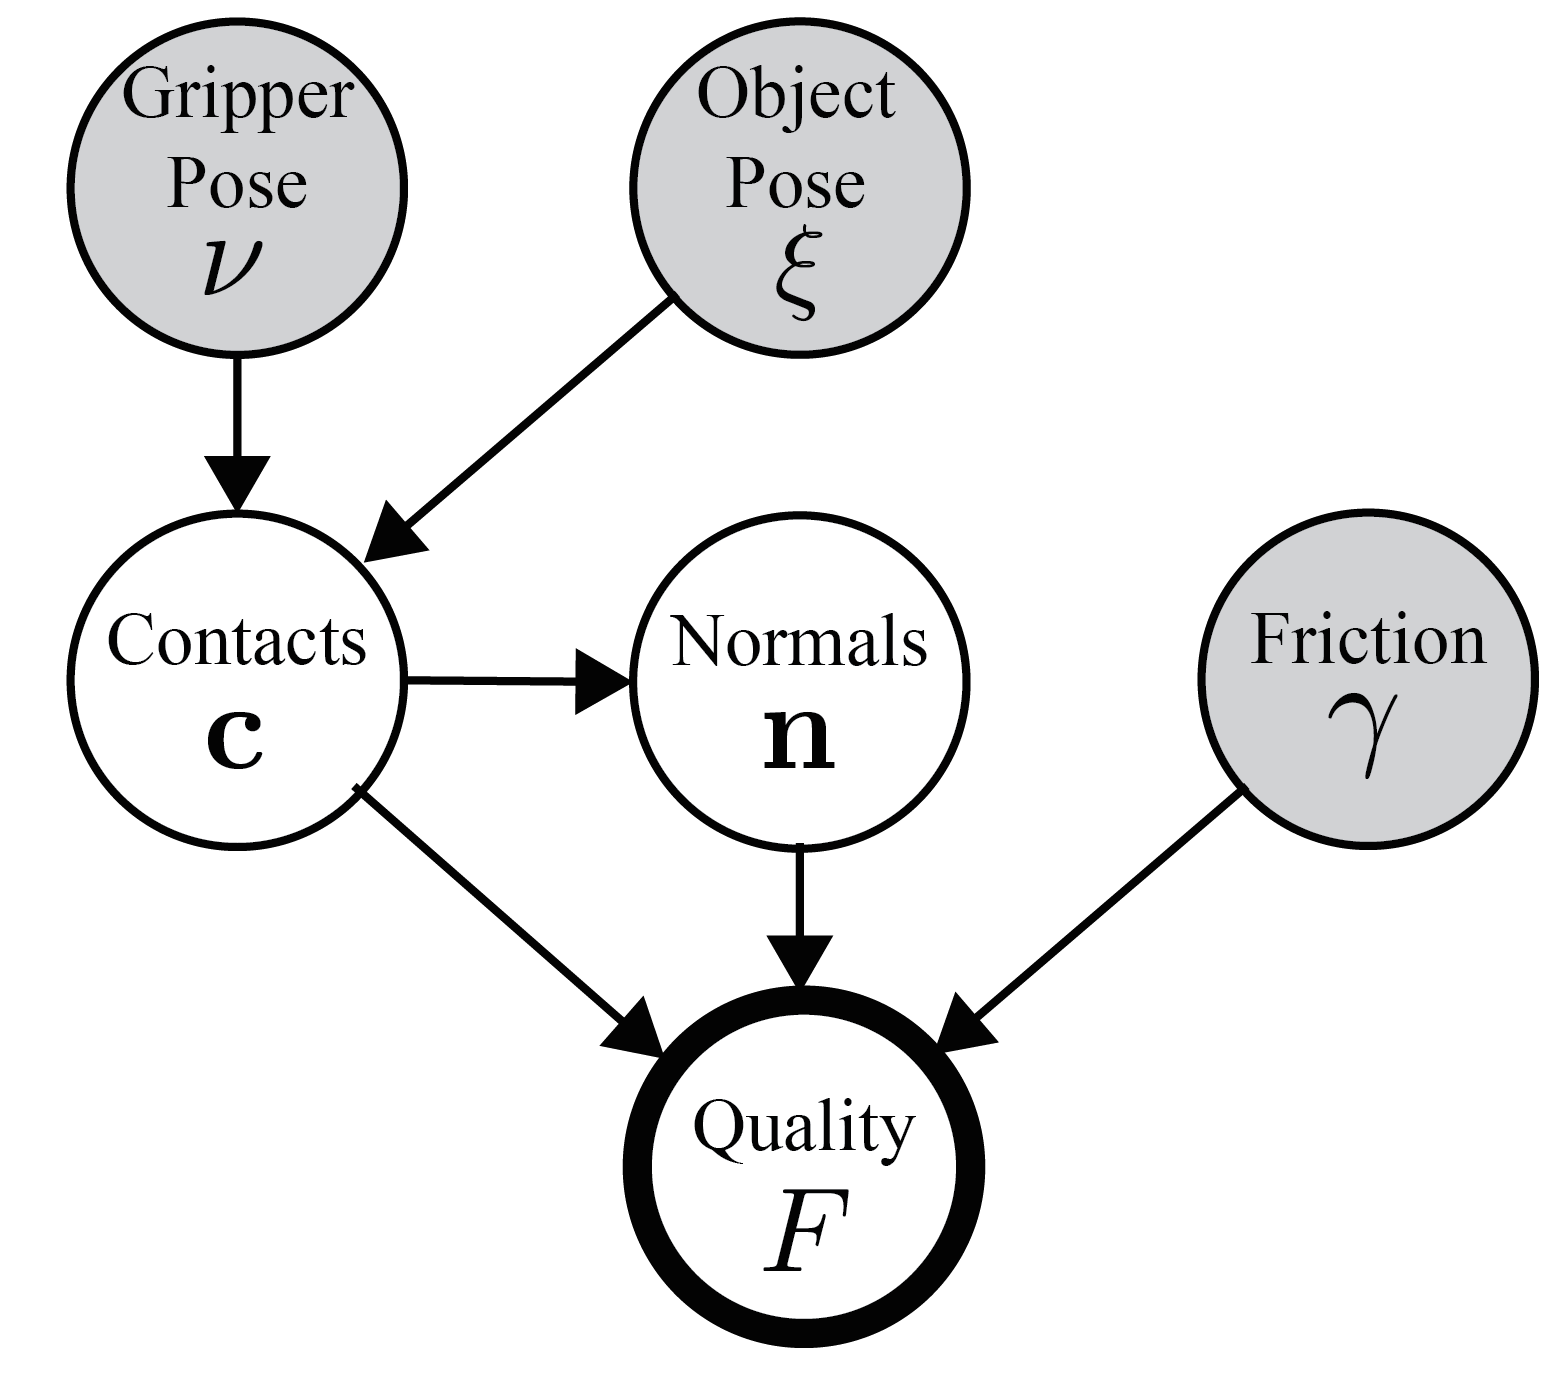
\includegraphics[scale=0.5]{figures/illustrations/dexnet_graphical_model_simple.png}
\caption{A graphical model describing the relationships between known uncertain parameters (shaded gray) such as object pose and the force closure random variable $F$.}
\figlabel{graphical-model}
\vspace*{-15pt}
\end{figure}

\subsection{Objective}
The probability of force closure for a grasp $\bg$ on object $\mO$ is
%\vspace{-2ex}
\begin{align*}
	P_F(\bg, \mO) = \mathbb{P}\left(F = 1 \mid \bg, \mO, \xi, \nu, \gamma \right).
\end{align*}
\noindent We are interested in finding the candidate grasp that maximizes the probability of force closure $P_F(g)$~\cite{kim2012physically, laskey2015bandits, mahler2015gp, weisz2012pose} subject to these sources of uncertainty over a budgeted maximum number of samples $T$.
To perform this as quickly as possible we formulate this as a maximization over the sum of the true $P_F$ for the grasps sampled at iteration $t$, where $I(i)$ denotes the grasp selected at time $t$~\cite{laskey2015bandits}:

\vspace{-2ex}
\begin{align}
	\underset{g_{I(1)}, ..., g_{I(T)} \in \mG}{\text{maximize }} \sum \limits_{t=1}^T P_F(g_{I(t)}). \label{eq:objective}
\end{align}

As the maximization over the continuous space $\mG$ is computationally expensive, past work has solved this objective using a discrete set of $K$ candidate grasps $\Gamma = \left\{ \bg_1, ..., \bg_K \right\}$ where $\Gamma$ is set by sampling grasp centers from a Gaussian with mean at the object center~\cite{laskey2015bandits} or using heuristics specific to parallel-jaw grippers such as antipodality~\cite{mahler2015gp}.
However, even with a discrete set of candidates, fully evaluating $P_F(\bg)$ for any grasp requires an expensive integration over possible contact locations between the grasp and surface and the surface normals at these contacts~\cite{mahler2015gp}.
Thus, past research has evaluated the probability of force closure using Monte-Carlo integration~\cite{kehoe2012estimating, kehoe2012toward, weisz2012pose}, approximating the expression by minimzing uncertainty at the contact locations~\cite{mahler2015gp}, and using Multi-Armed Bandit (MAB) algorithms to jointly evaluate $P_F(\bg)$ using Monte-Carlo integration while allocating samples to more promising grasps.
In this work, we extend the MAB model of~\cite{laskey2015bandits} to model similarities between grasps and prior objects in Dex-Net to further accelerate convergence.

%\TODO{Switch to task-based quality metric (e.g. resiting gravity)? I think it would be more compelling but doesn't seem to have much precedent under uncertainty}